\documentclass[final]{beamer}
\mode<presentation>{\usetheme{I6dv}}
%\usefonttheme[onlymath]{serif}
\usefonttheme{default}

\usepackage{microtype}
\usepackage{fixltx2e}

%\usepackage[T1]{fontenc}
%\usepackage{lmodern}

\usepackage[orientation=landscape,size=a1]{beamerposter} 
\usepackage{exscale}
\usepackage{booktabs, array}
\usepackage[english]{babel}
\usepackage[latin1]{inputenc}
\usepackage{amsmath,amsthm, amssymb, latexsym}
\usepackage{graphicx}
\usepackage[center,labelformat=empty, font=normal]{caption}
\usepackage[labelformat=empty, font=normal]{subcaption}


%\beamertemplategridbackground[1em]

%\usepackage{enumitem}
%\setitemize{itemsep=.5em}
%\setlength{\itemsep}{5em}

\begin{document}
\begin{frame}{ }
    \begin{columns}[t]
        \begin{column}{.26\linewidth}

            \begin{block}{Introduction}
                \begin{itemize}
                    \itemsep.5em
                    \item transportation forecasting model
                    \item mathematically describes the behaviour of traffic
                    \item people wish to travel on shortest path with least travel time
                    \item \alert{goal}: find a \alert{faster} algorithm for solving the \alert{shortest path} problem between origins and a destinations in transportation network
                \end{itemize}
            \end{block}

            \hspace{25em}

            \begin{block}{Traffic Assignment}
                \begin{itemize}
                    \itemsep.5em
                    \item \alert{Traffic Assignment (TA)} deals with selection of \alert{shortest path} for everyone in the network to \alert{minimise} their \alert{travel times}
                    \item a \alert{non-linear} problem, travel times increase dramatically when \alert{congestion} happens
                    \item an \alert{iterative algorithm} called \alert{Path Equilibration (PE)} algorithm is used to solve TA
                    \item \alert{PE} requires to find \alert{millions} of \alert{shortest paths}
                    \item solve shortest path faster to speed up TA 
                    \item benefit transportation modelling
                \end{itemize}
            \end{block}

            \hspace{25em}

            \begin{block}{Shortest Path Algorithms}
                \begin{itemize}
                    \itemsep.5em
                    \item find path with least distance in network
                    \item scan nodes in network in some order until destination is found
                    \item need a data structure called \alert{priority queue} to keep the scanned nodes in sequence so the next node to scan can be easily found
                \end{itemize}
            \end{block}

            \hspace{25em}

            \begin{block}{Faster in Traffic Assignment}
                \begin{itemize}
                    \itemsep.5em
                    \item in PE, can \alert{avoid} shortest path calculations to speed up overall performance
                    \item use shortest path from previous iteration if calculation in current iteration is avoided
                    \item first strategy: avoid the \alert{next few} iterations if the shortest path of the \alert{previous two} iterations are \alert{identical}
                    \item second strategy: \alert{randomly avoid} the next shortest path calculation in the hope that path of \alert{previous and current} iteration are \alert{identical}
                \end{itemize}
            \end{block}

        \end{column}
        \begin{column}{.4\linewidth}

            \begin{block}{Search Areas of Shortest Path Algorithms}
                \begin{itemize}
                    \itemsep.5em
                    \item performance of shortest path algorithms is heavily dependent on the \alert{search area}
                    \item \alert{search less} area should be \alert{faster}
                    \item the following figures demonstrate search areas of the implemented shortest path algorithms on a \alert{medium sized} network with $546$ nodes and $2{,}950$ arcs
                \end{itemize}
                \vspace{1em}
                \begin{figure}
                    \centering
                    \begin{subfigure}{.5\linewidth}
                        \centering
                        {\bfseries Dijkstra's algorithm }
                        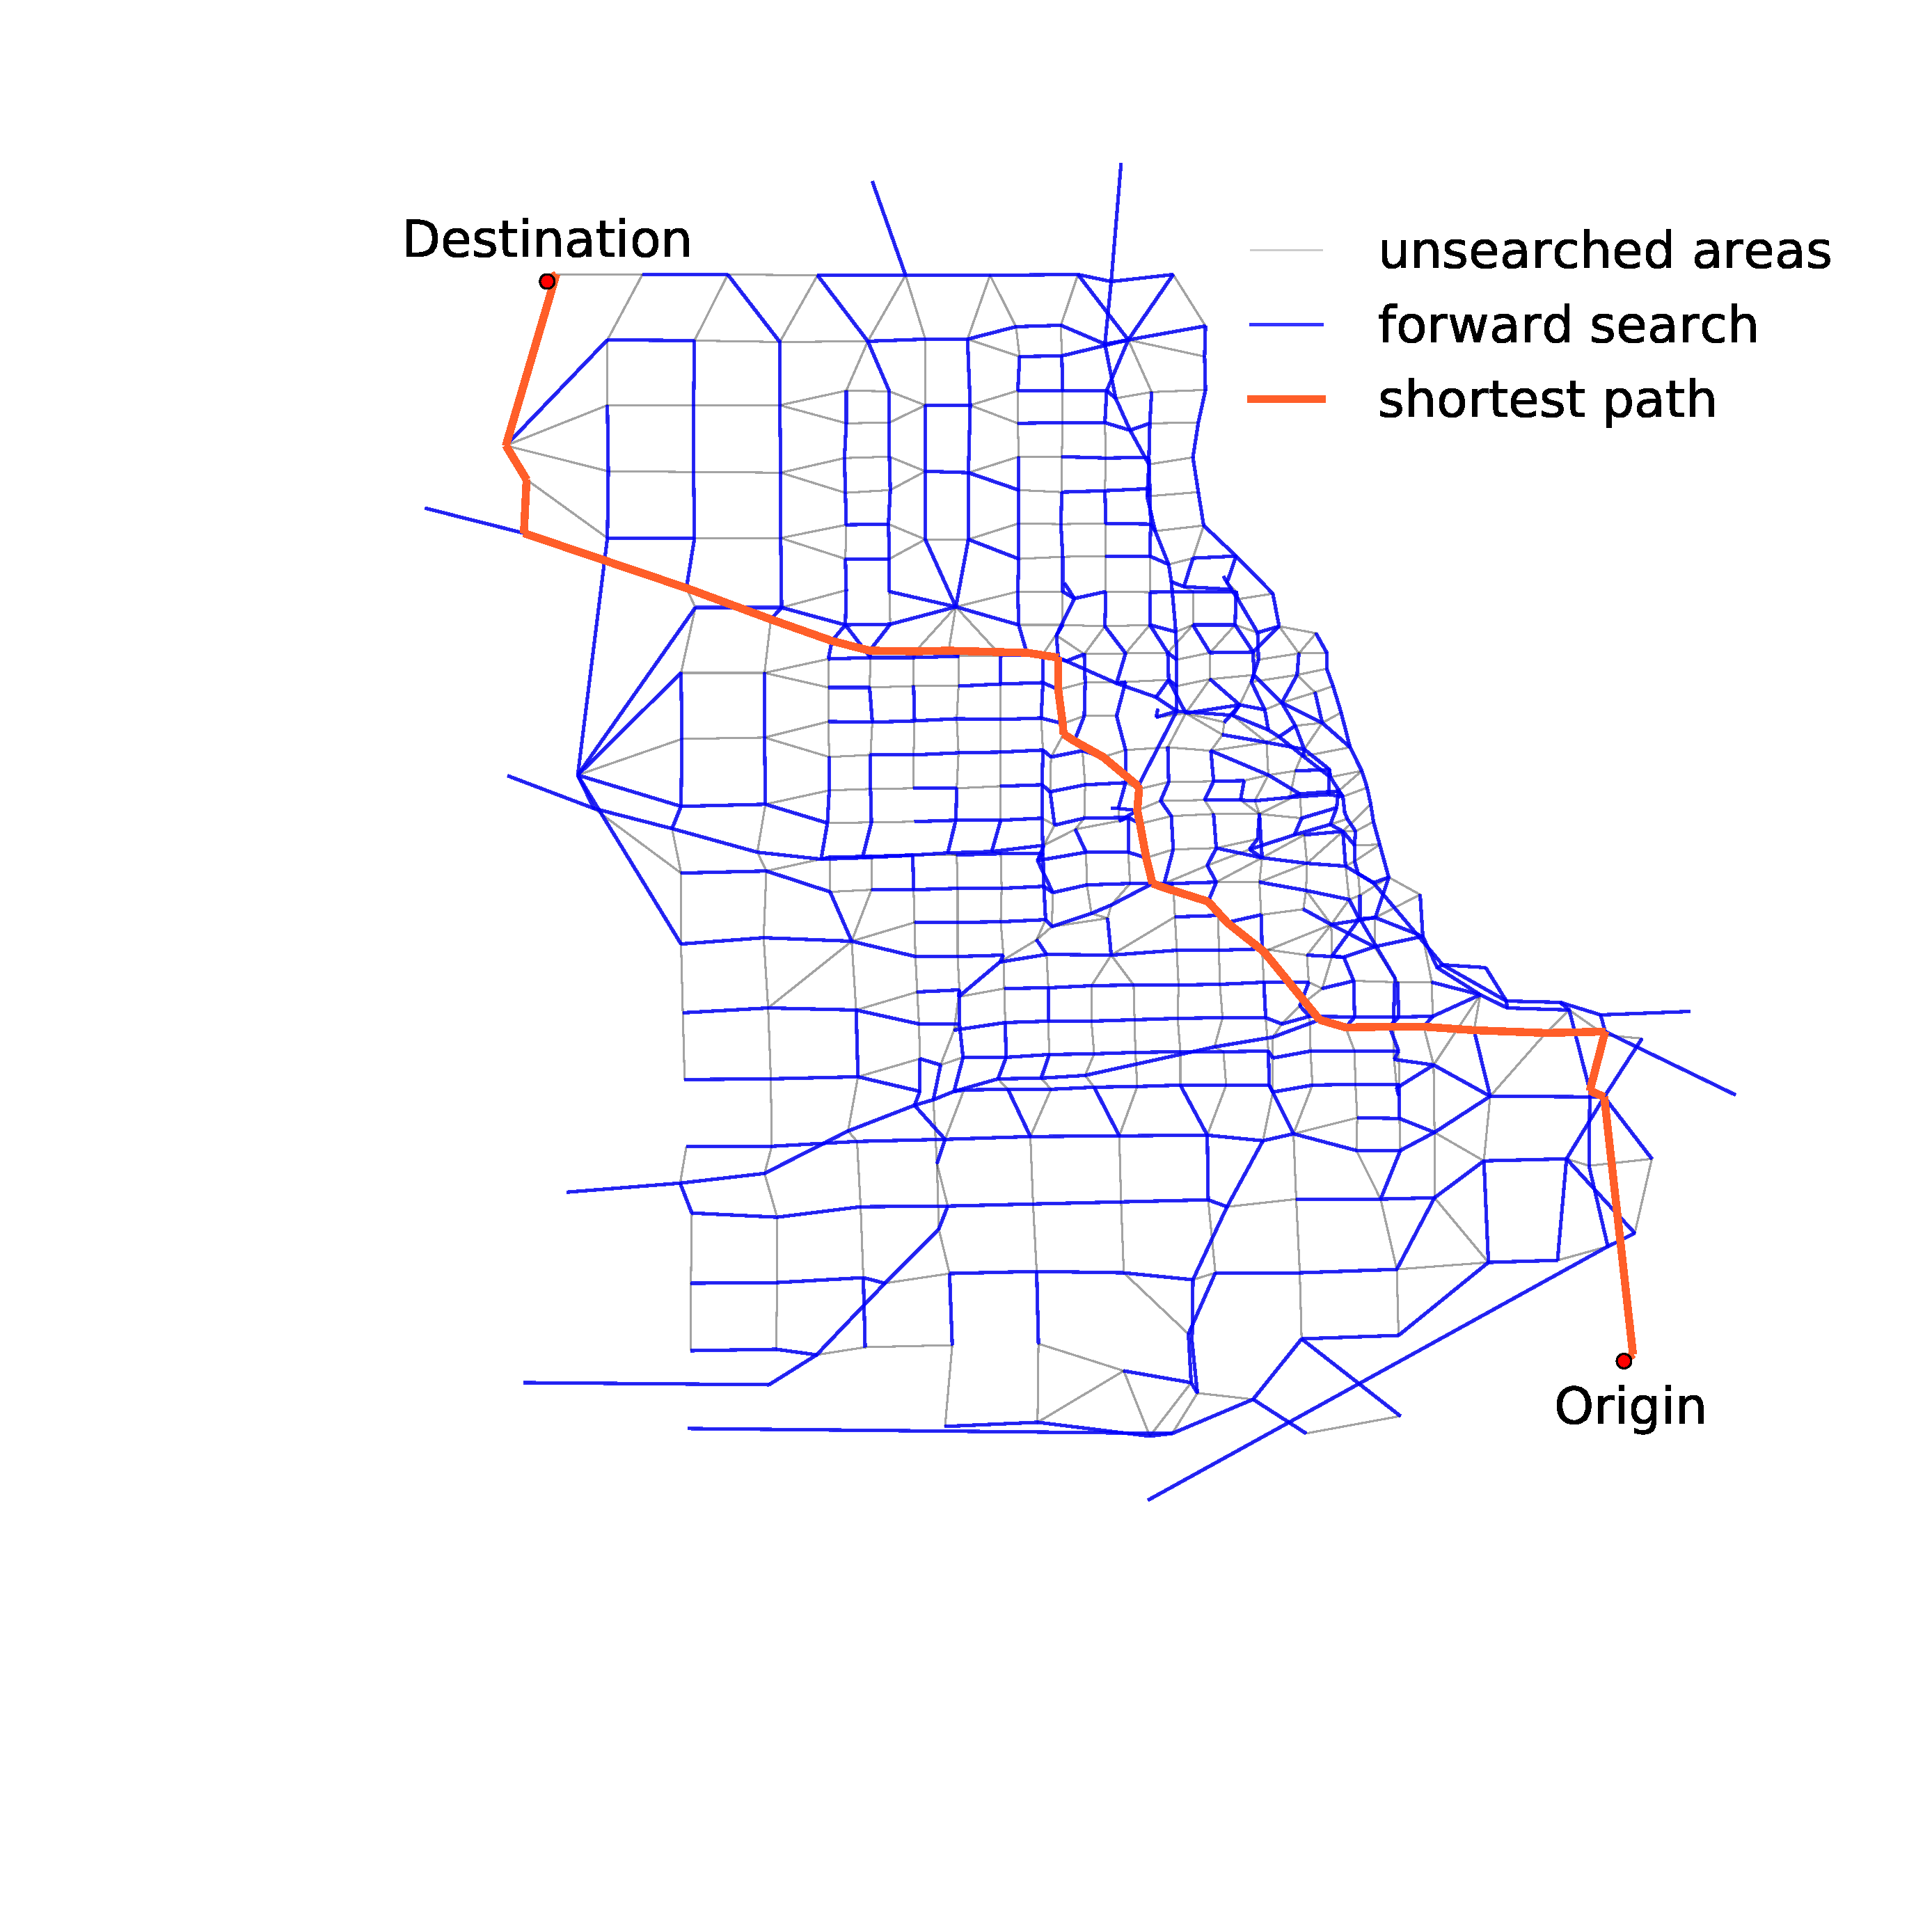
\includegraphics[width=\linewidth,trim=120px 280px 48px 60px,clip]{img/dijkstra}
                        \caption{searches the \alert{entire network}}
                    \end{subfigure}%
                    \begin{subfigure}{.5\linewidth}
                        \vspace{.1em}
                        \centering
                        {\bfseries Bidirectional Dijkstra's algorithm}
                        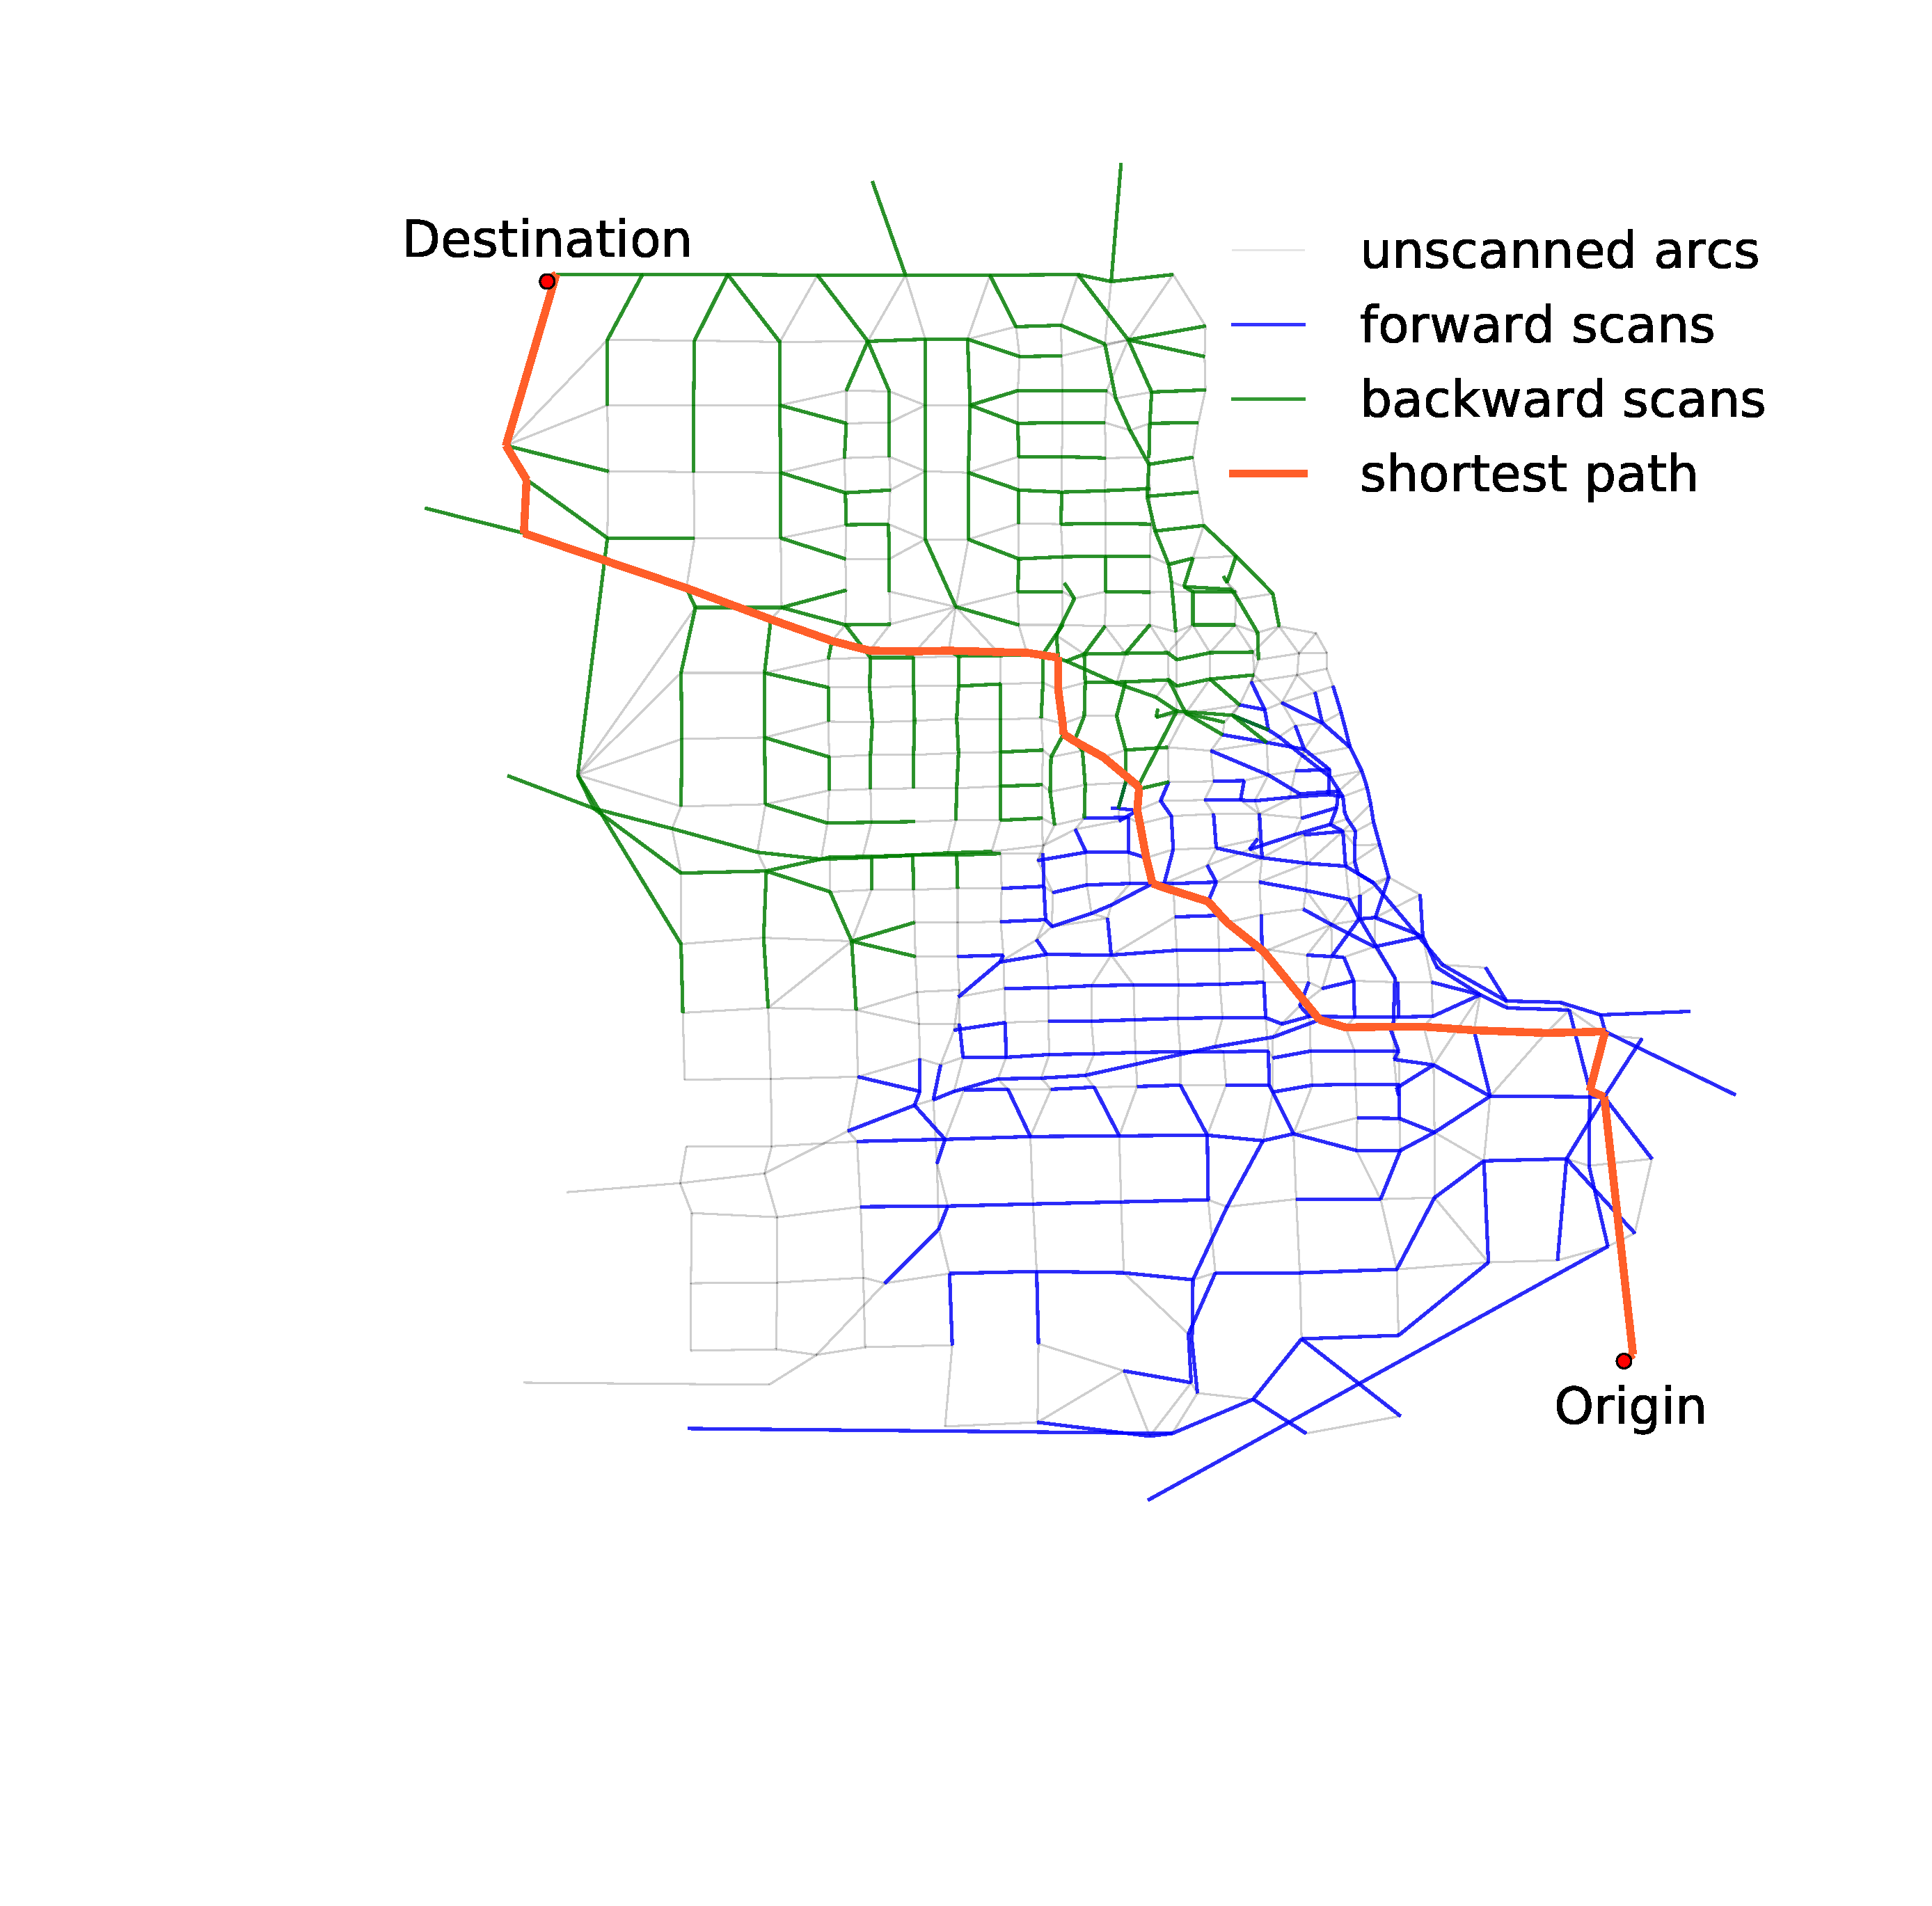
\includegraphics[width=\linewidth,trim=120px 280px 48px 60px,clip]{img/dijkstra_bidirect}
                        \caption{searches from \alert{both ends simultaneously}}
                    \end{subfigure}
                    \begin{subfigure}{.5\linewidth}
                        \centering
                        {\bfseries A* Search}
                        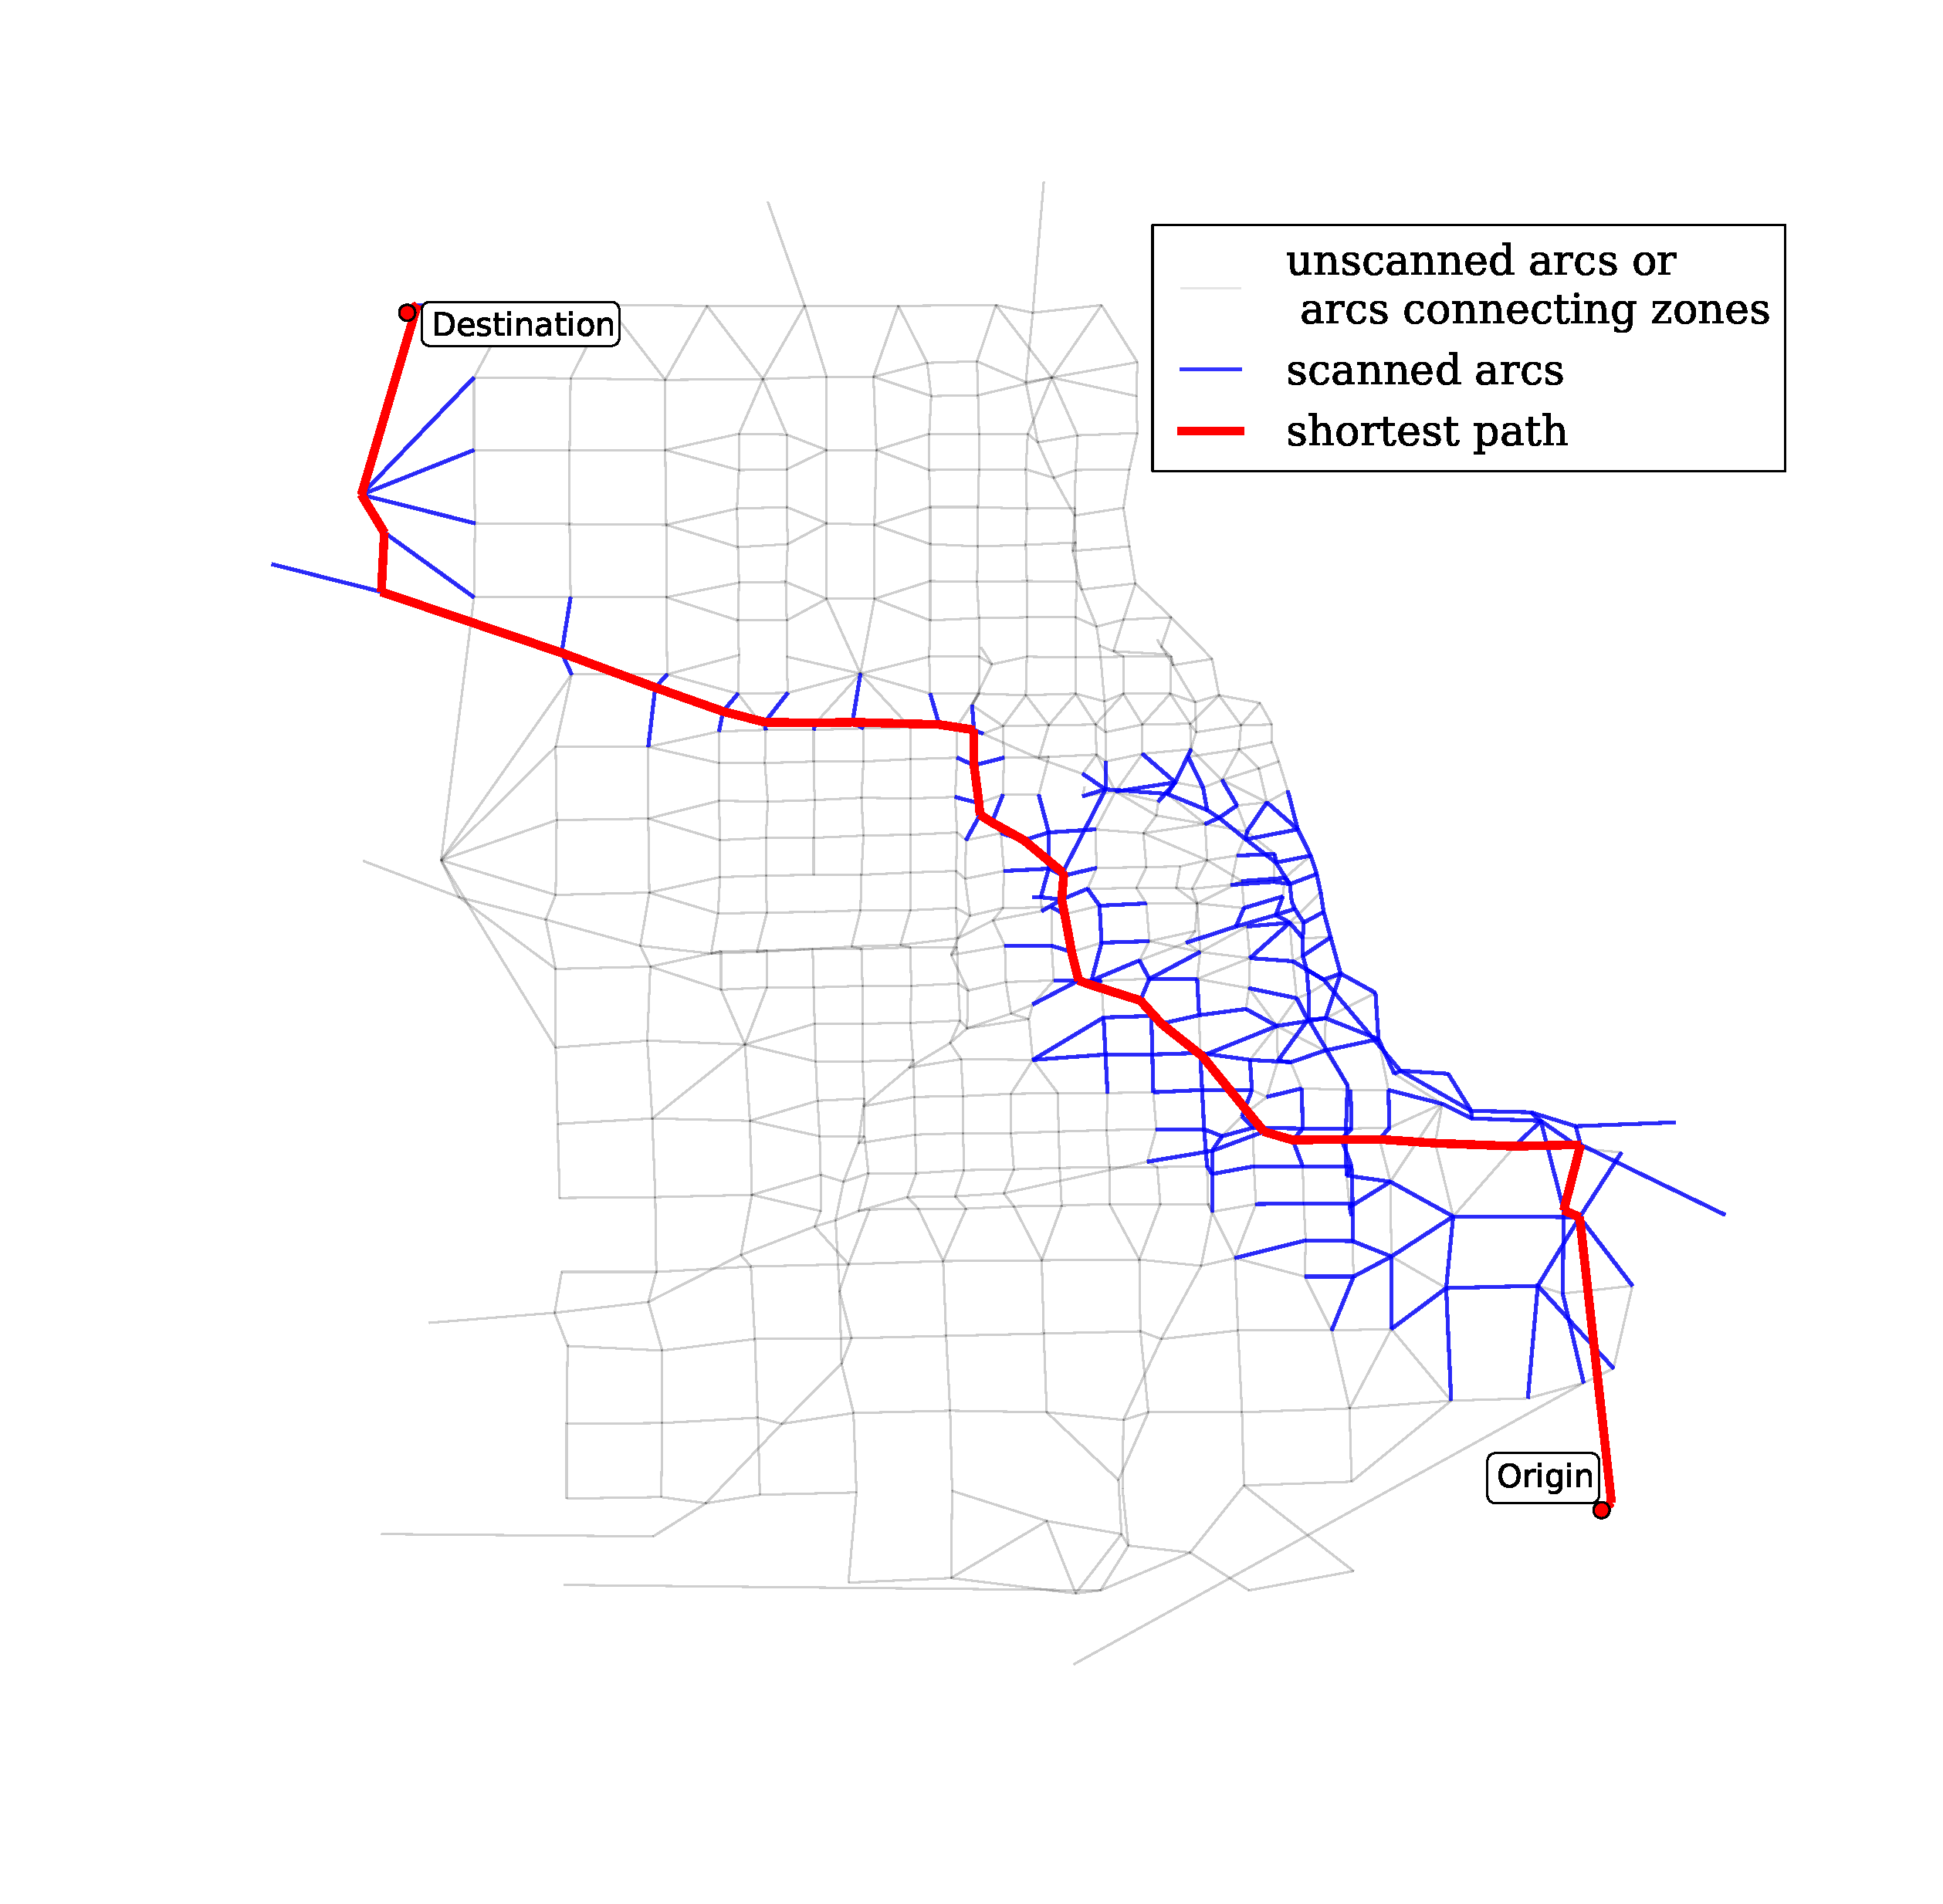
\includegraphics[width=\linewidth,trim=120px 280px 48px 60px,clip]{img/astar}
                        \caption{searches \alert{along the expected} shortest path}
                    \end{subfigure}%
                    \begin{subfigure}{.5\linewidth}
                        \vspace{1.3em}
                        \centering
                        {\bfseries Bidirectional A* Search}
                        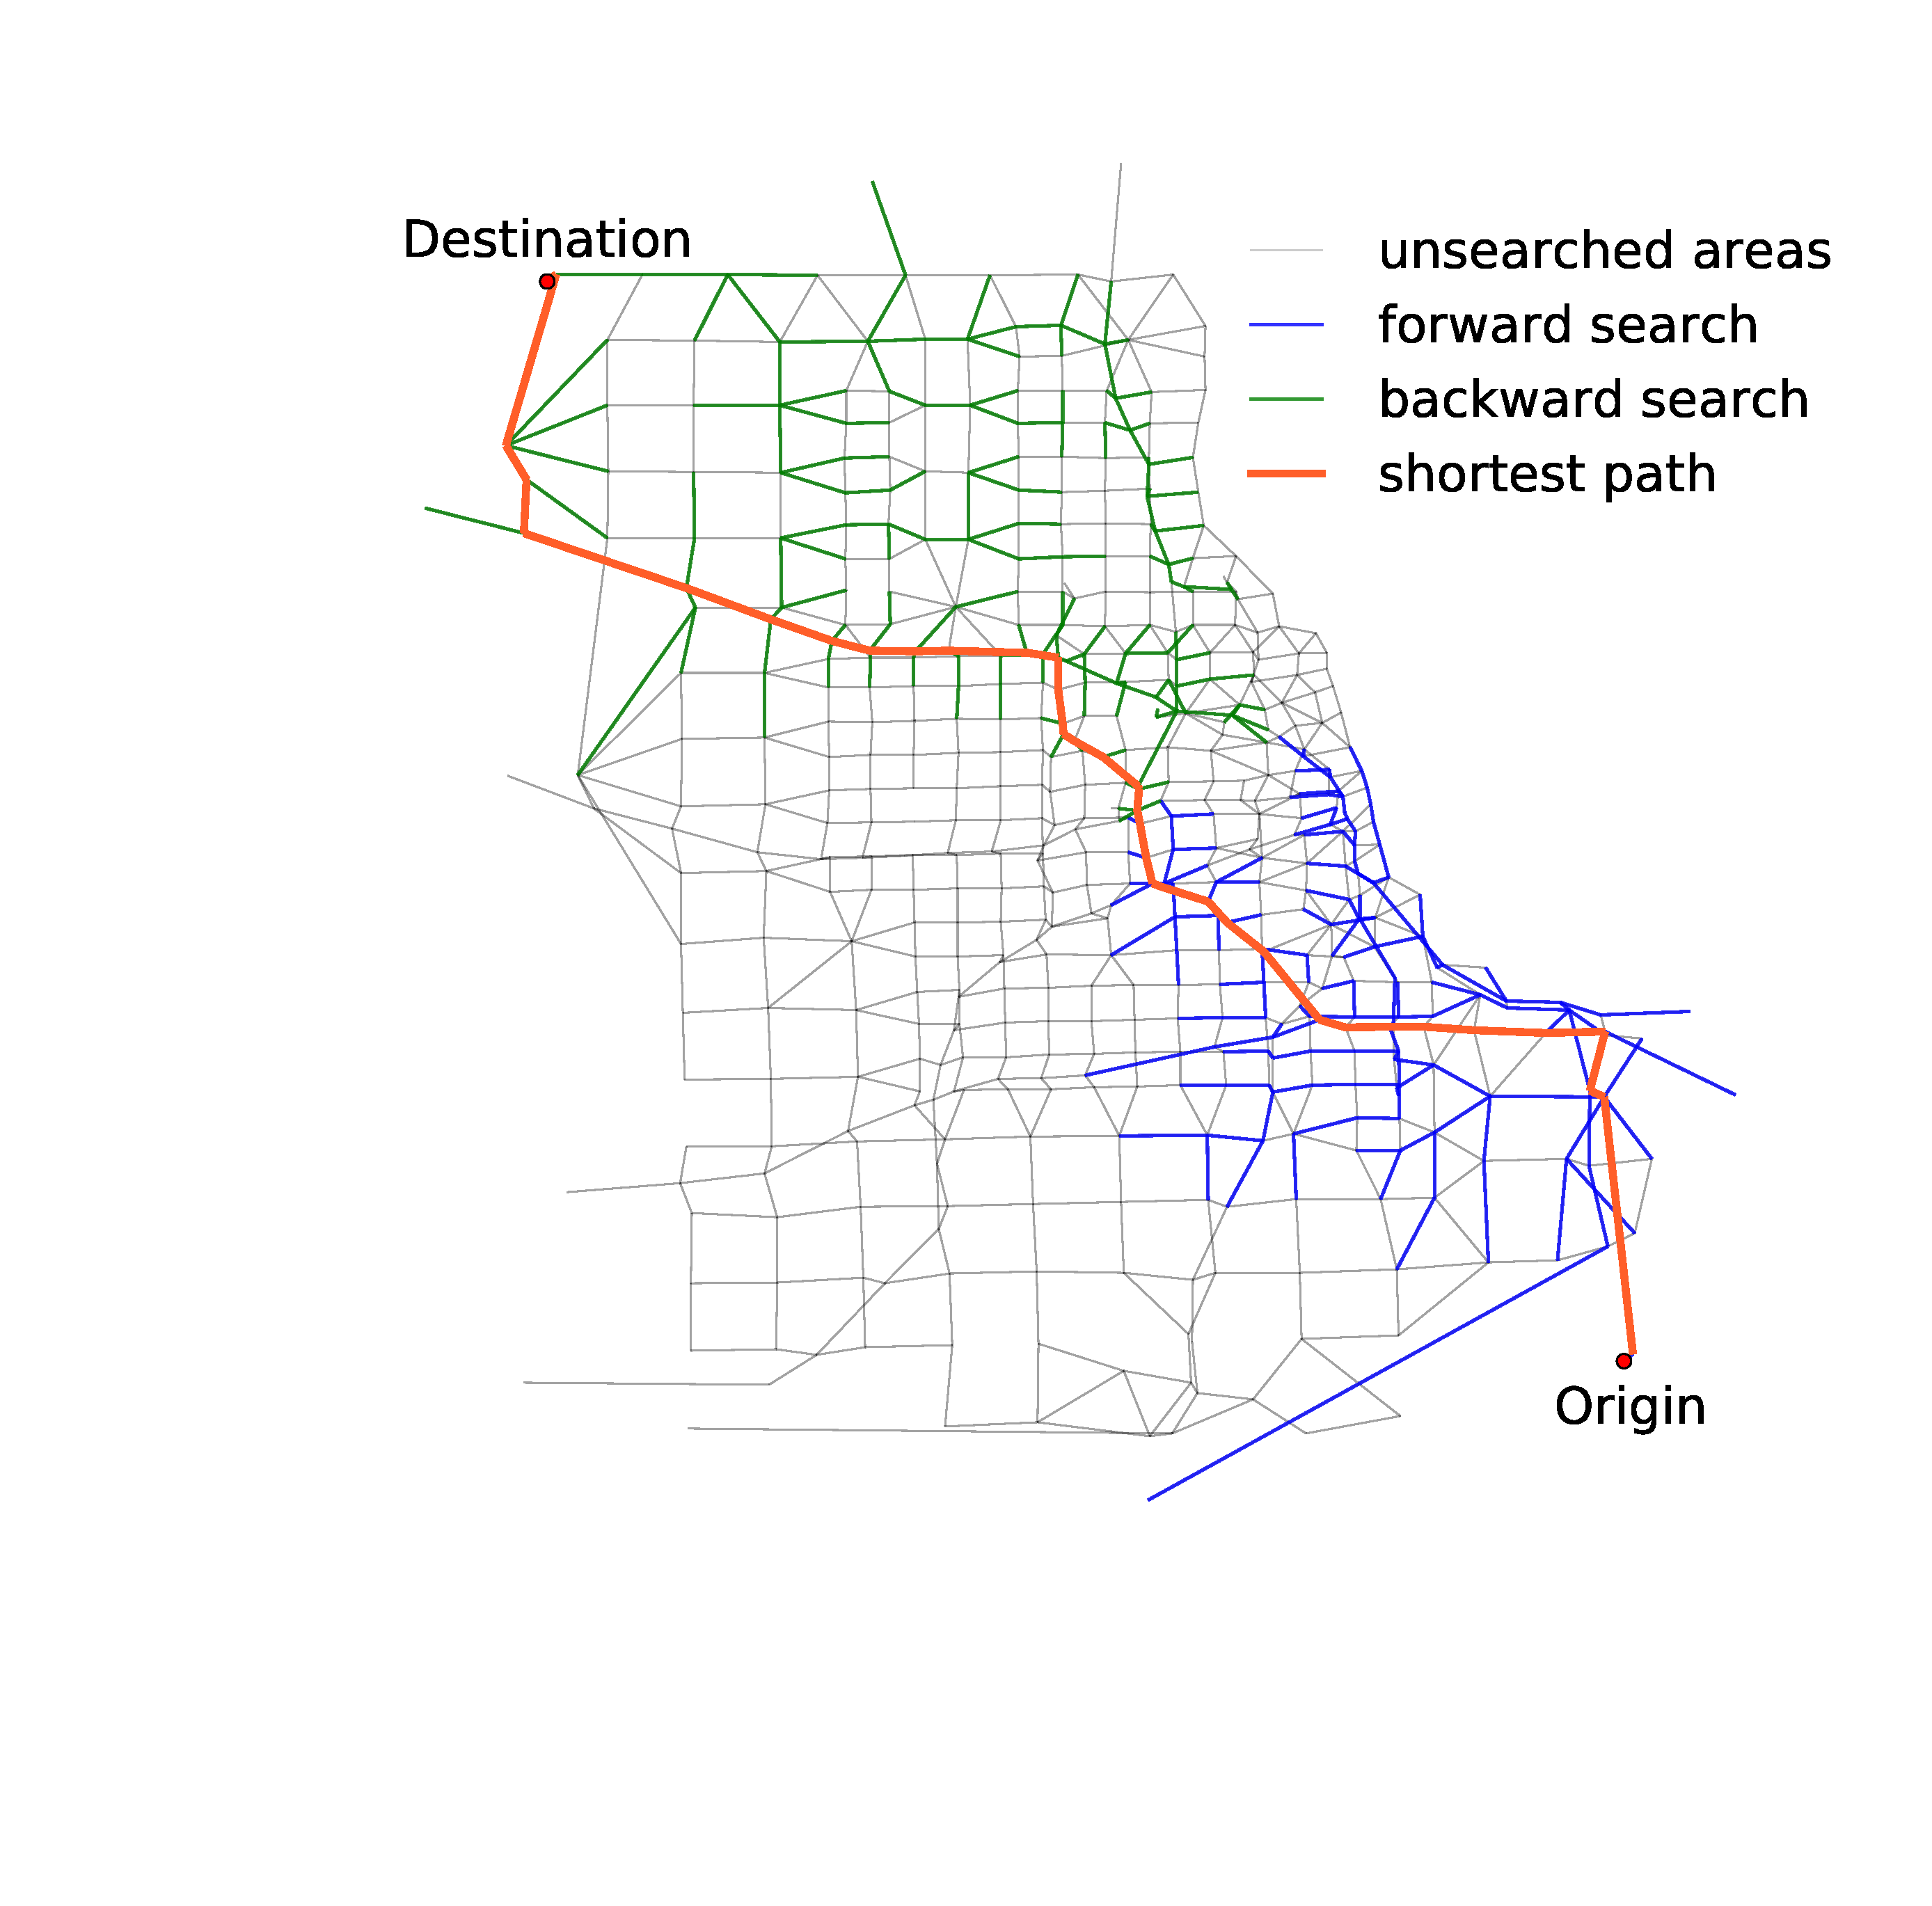
\includegraphics[width=\linewidth,trim=120px 280px 48px 60px,clip]{img/astar_bidirect}
                        \caption{searches \alert{along the expected} shortest path from \alert{both ends simultaneously}} 
                    \end{subfigure}
                \end{figure}
                \begin{itemize}
                    \itemsep.5em
                    \item Dijkstra's algorithm searches the most
                    \item bidirectional Dijkstra's algorithm searches slightly less
                    \item \alert{A* search searches the least area}
                    \item bidirectional A* search searches more than unidirectional A*
                \end{itemize}
            \end{block}

        \end{column}
        \begin{column}{.26\linewidth}
            \begin{block}{Results on Medium Sized Network}
                \begin{itemize}
                    \itemsep.5em
                    \item tested \alert{8 different priority queues}, implemented \alert{4 shortest path algorithms} and experimented \alert{2 strategies} for traffic assignment
                \end{itemize}
                \begin{figure}
                    \centering
                    {\bfseries \qquad Run times of Dijkstra's algorithm\\ \qquad using different priority queues}
                    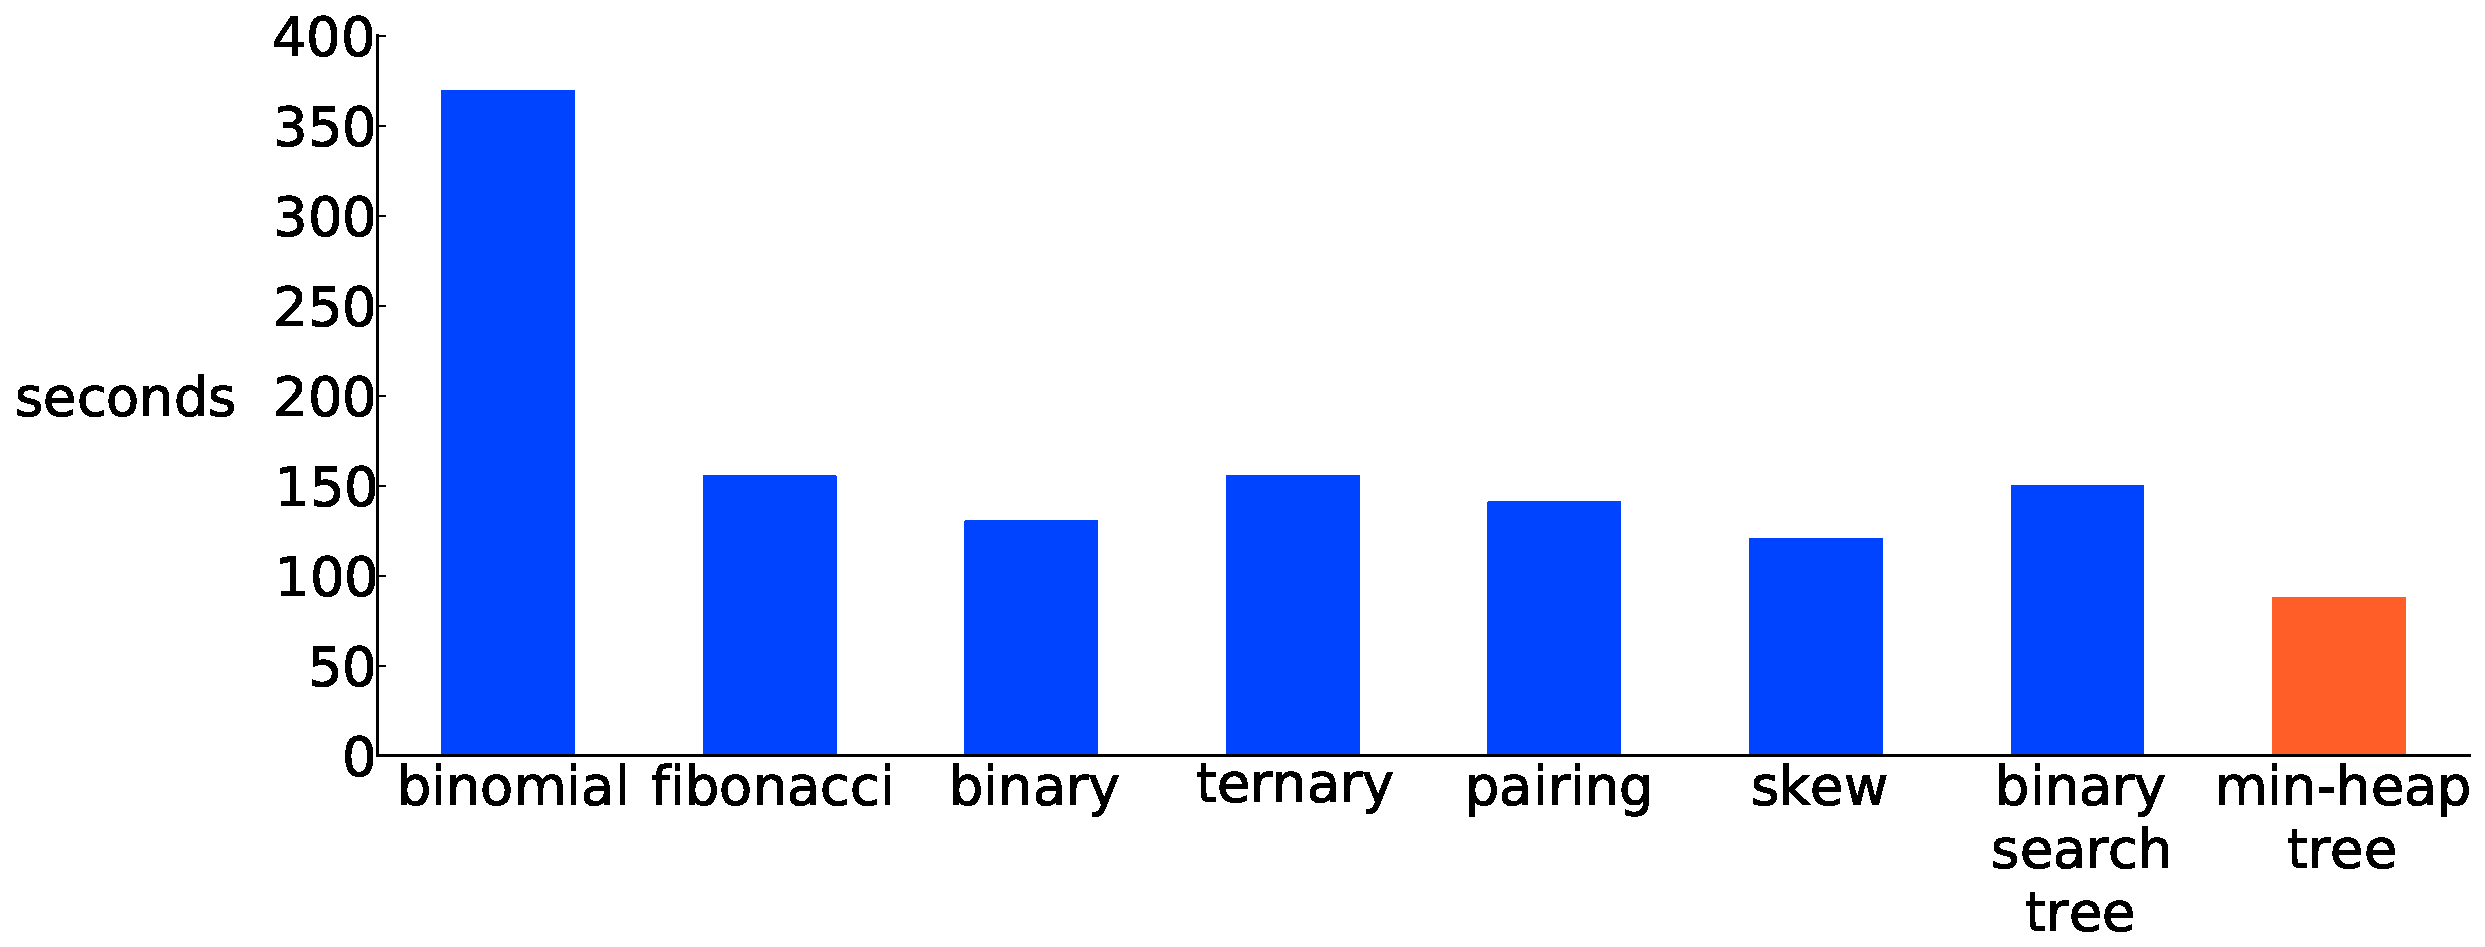
\includegraphics[width=\linewidth]{img/pq_runtime}
                \end{figure}
                \begin{figure}
                    \centering
                    {\bfseries \qquad Run times of shortest path algorithms\\ using min-heap tree}
                    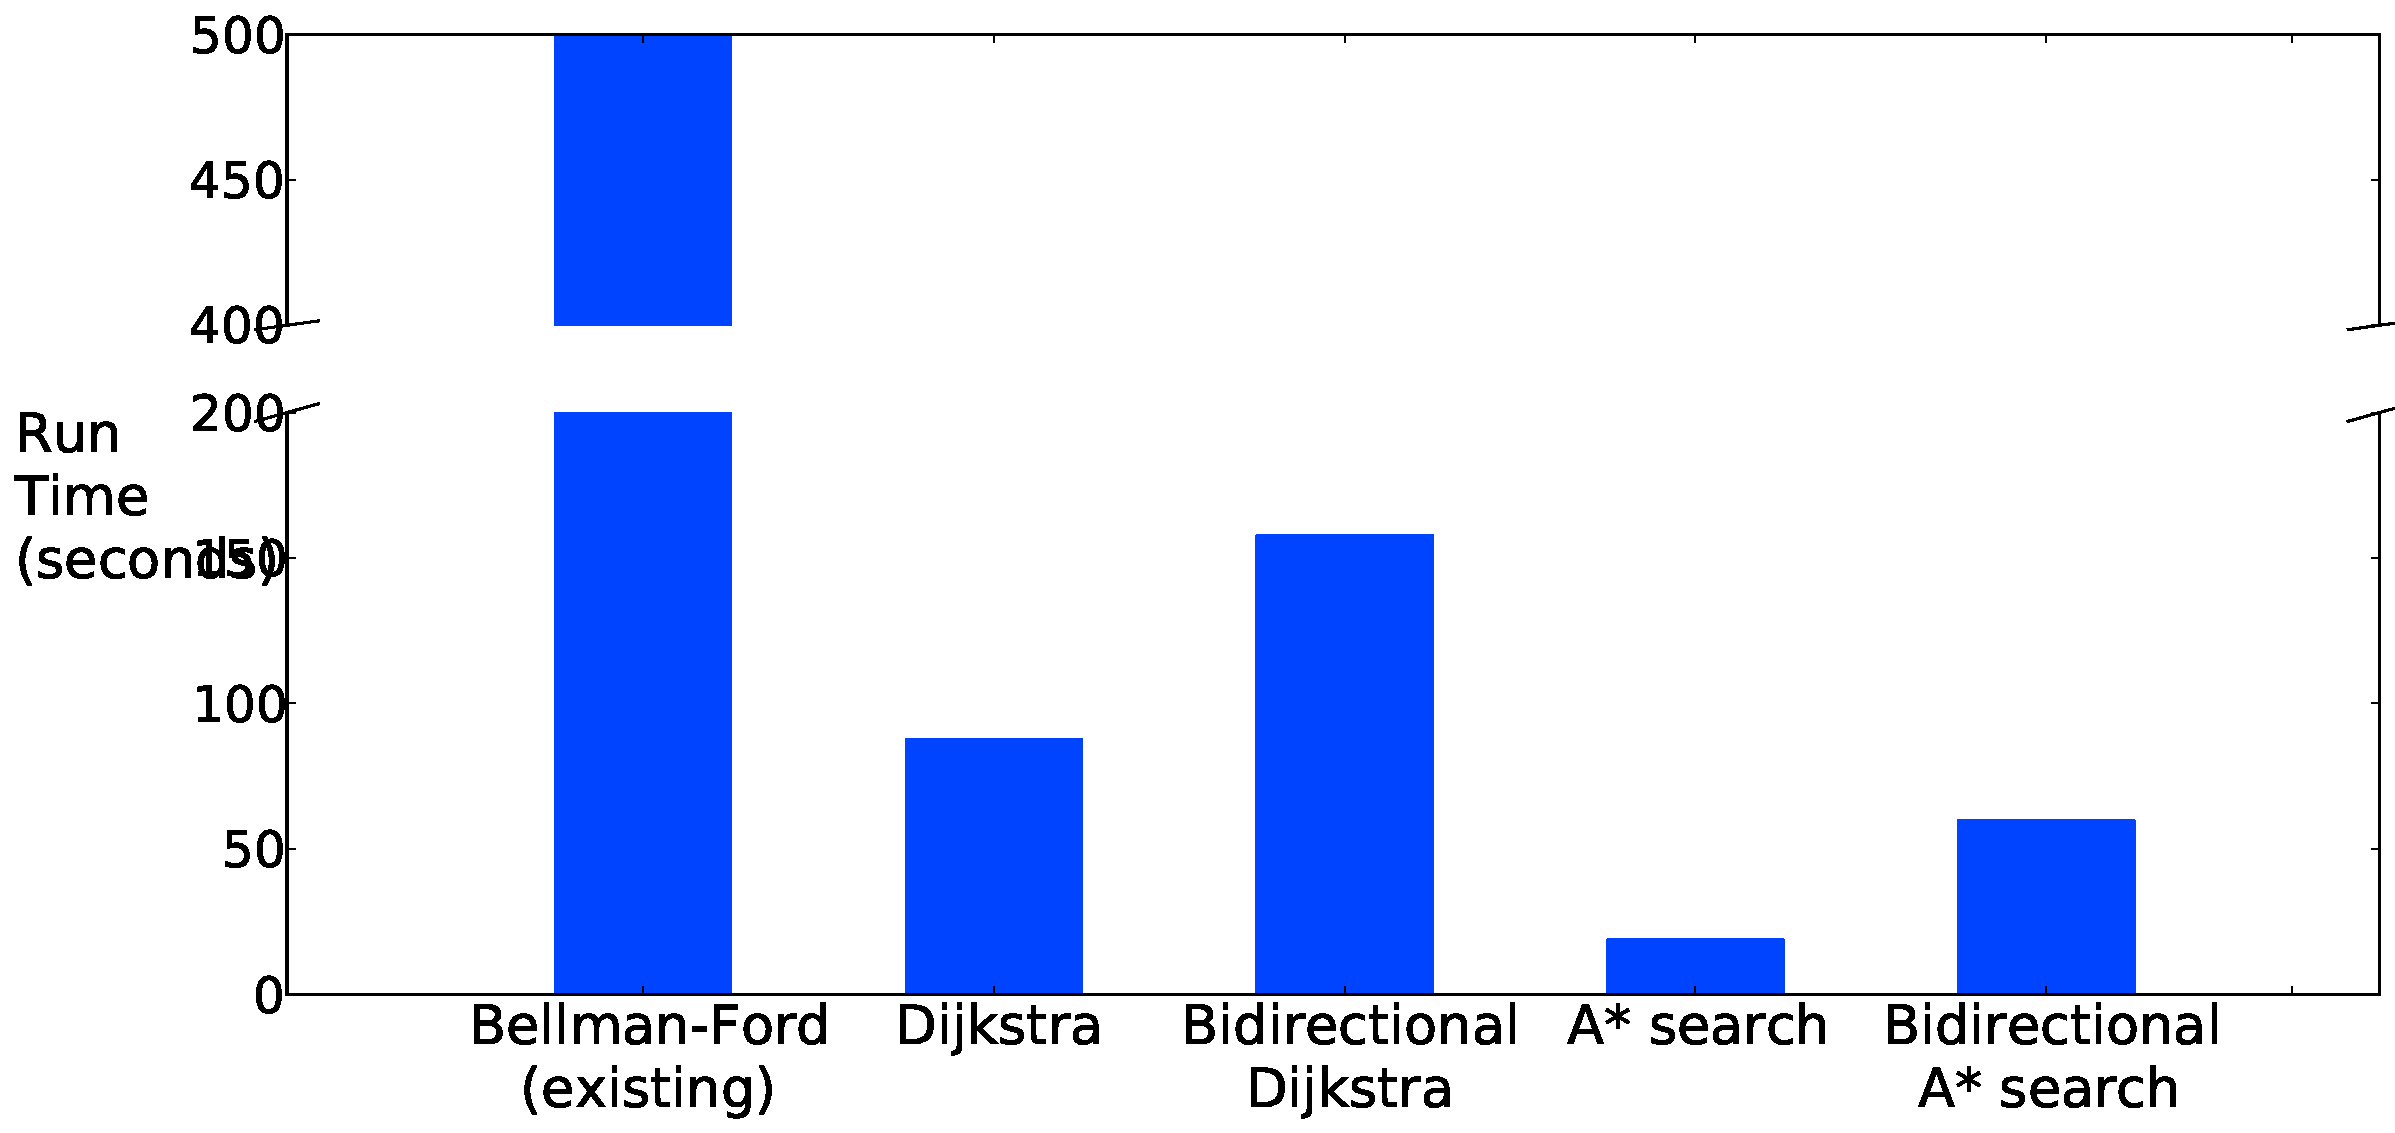
\includegraphics[width=\linewidth]{img/runtime}
                \end{figure}
                \begin{figure}
                    \centering
                    {\bfseries \qquad Run times of A* search using avoiding\\ \qquad shortest path calculation strategies}
                    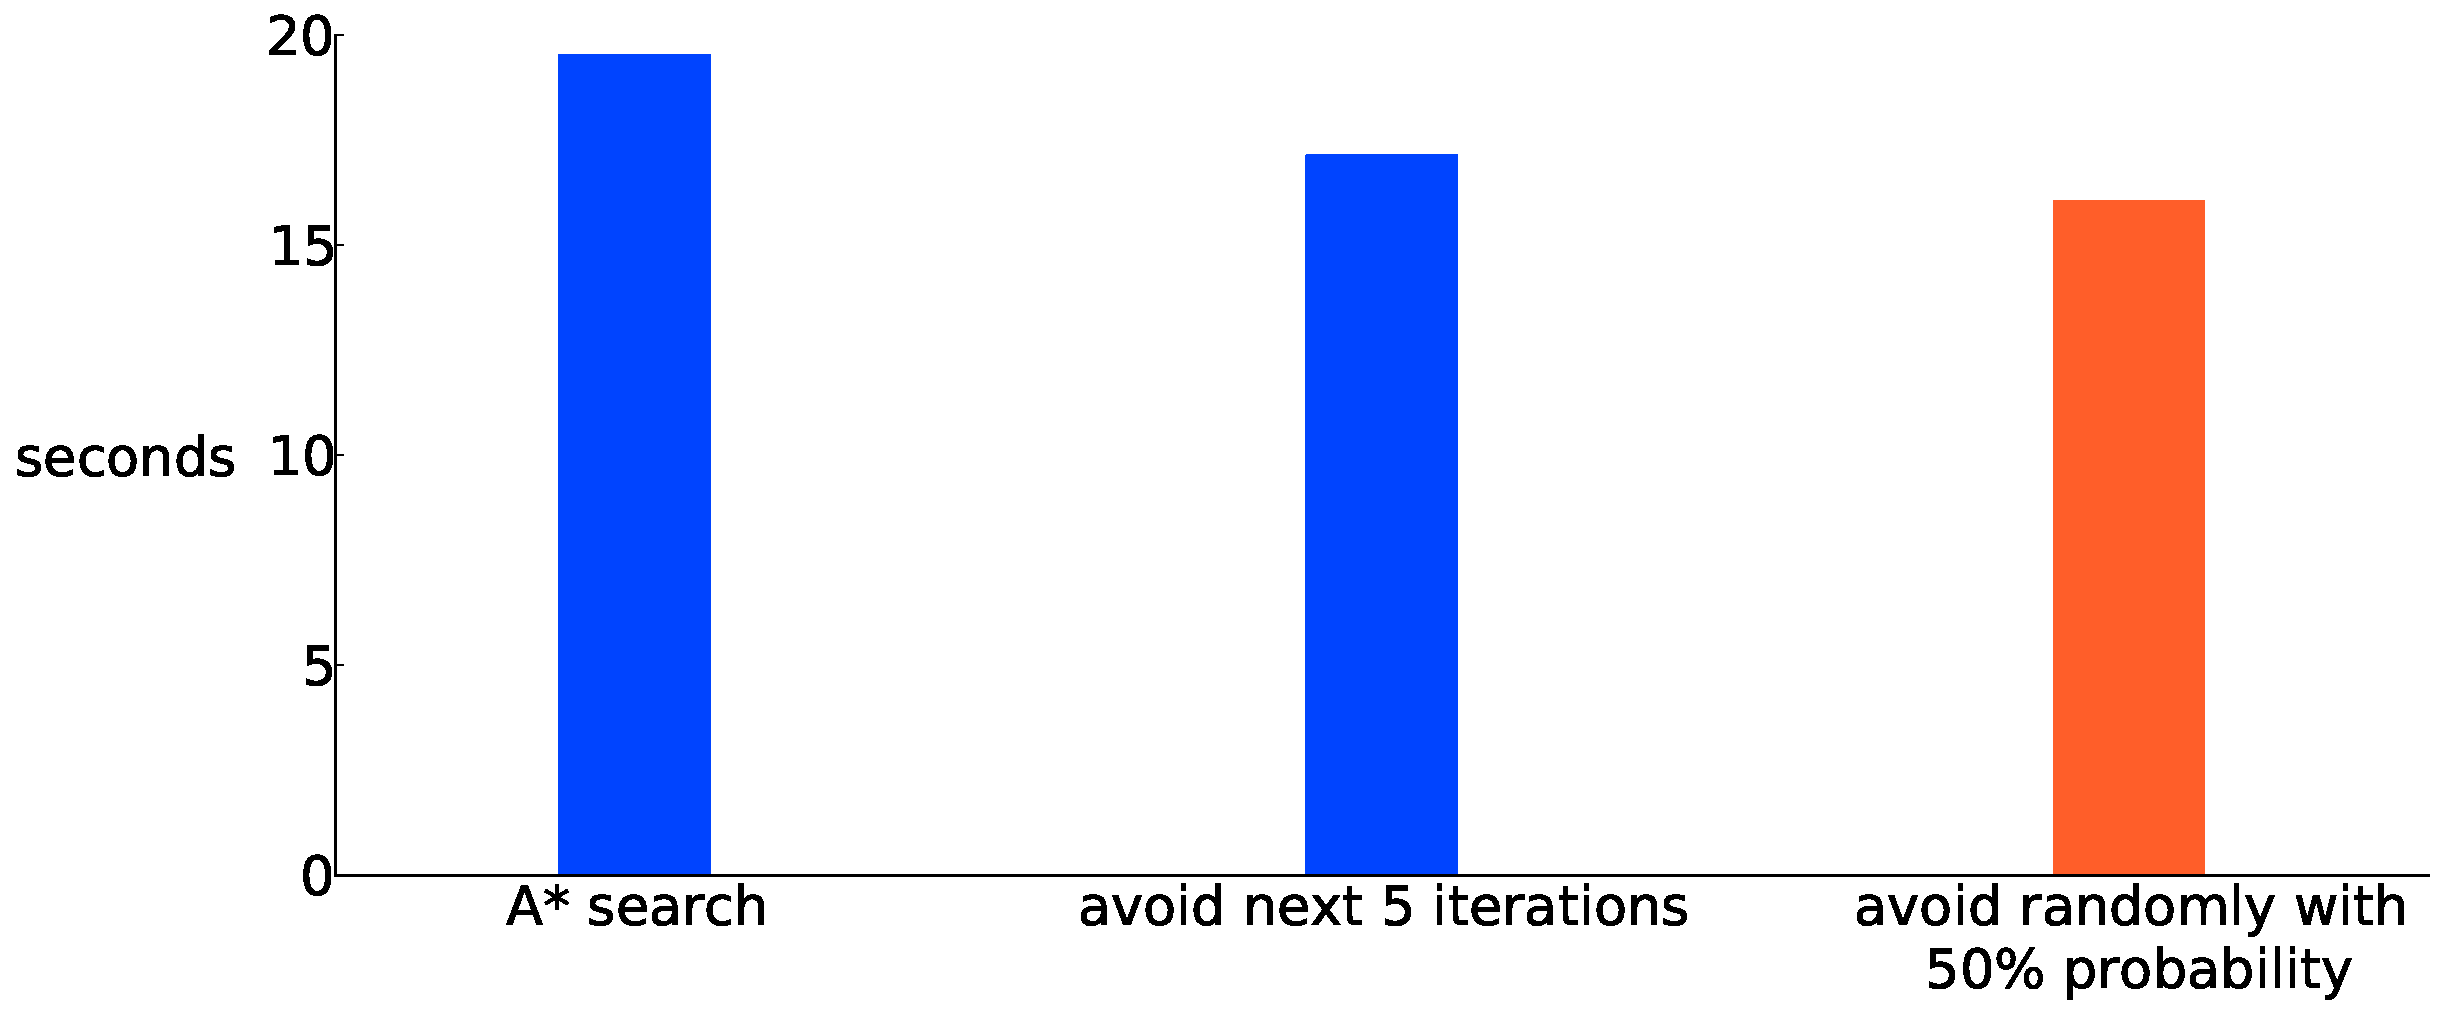
\includegraphics[width=\linewidth]{img/random_runtime}
                \end{figure}
            \end{block}
            \begin{block}{Conclusion}
                \begin{itemize}
                    \itemsep.5em
                    \item \alert{best performance}: A* search algorithm using min-heap tree with random avoiding strategy
                    \item overall more than \alert{3000\% improvement} compared to the existing shortest path algorithm
                \end{itemize}
            \end{block}
        \end{column}
    \end{columns}
\end{frame}

\end{document}
